\documentclass[bachelor, english]{algothesis}
% possible types: bachelor, master, zula (seminar, practical)
% Für Seminararbeiten und Praktikumsberichte die Vorlage my-seminar-praktikum.tex verwenden!
% possible languages: english, german

\usepackage[utf8]{inputenc}
\usepackage{svg}
\usepackage{hyperref}
\usepackage{xtab}
\usepackage[T1]{fontenc}
\usepackage{lmodern}
\usepackage{caption}
\usepackage{algpseudocode}
\usepackage{booktabs} 
\usepackage{longtable}
\captionsetup[figure]{name=Fig.}
\addto\captionsenglish{
    % Second argument is singular, third is plural
    \crefname{figure}{figure}{figure}
    \Crefname{Figure}{Figure}{Figure}
    \crefname{table}{table}{table}
    \Crefname{Table}{Table}{Table}
    \crefname{chapter}{chapter}{chapter}
    \Crefname{Chapter}{Chapter}{Chapter}
}
\graphicspath{{figures/}}

%%%%%%%%%%%%%%%%%%%%%%%%%%%%%%%%%%%%%%%%%%%%%%%%%%%%%%%%%%%%%%%%%%%%%%%%%%
%%%%%%%%%%%%% Bitte nur ab hier Änderungen vornehmen %%%%%%%%%%%%%%%%%%%%%

\title{The Track Layout Problem from a SAT-Solving Perspective} % Geben Sie hier den Titel Ihrer Arbeit an.

\author{Simon Szulik} % Geben Sie Ihren Namen an.

\newcommand{\abgabedatum}{29. February 2024} % Hier wird das Abgabedatum angepasst

\supervisors{% Geben Sie die Namen aller Betreuenden an, getrennt durch das Makro '\and'
Jun.-Prof.\ Dr.\ Philipp Kindermann \and
Prof.\ Dr.\ Stefan Näher} 


\begin{document}

\begin{abstract}
In a track layout of a graph, nodes are arranged into sequences called tracks, where each sequence comprises an independent set of nodes, and edges connecting pairs of tracks form a set that does not intersect. In this bachelor thesis, we examine this well-known graph problem from a different perspective: we compare different SAT formulations and examine the usability and advantages of each. The focus is on developing and comparing different approaches to represent crossing edges. We have shown that a relational view of the node positions within the track layout is the more sensible approach. On this basis, we set up two approaches, which we then test and compare with 100 randomly selected test graphs of different sizes (10-100 nodes). The variants differ in their formulation, which ensures that two nodes are  are not on the same track. The evaluation showed that adding an extra variable drastically reduces the number of clauses, but at the expense of evaluation time. As a byproduct, we discover that the time required to create the clauses gradually decreases in percentage relevance as the number of nodes increases.
\end{abstract}

\begin{germanabstract}
In dem Track-Layout eines Graphen sind die Knoten in Sequenzen angeordnet, die Spuren genannt werden. Jede dieser Sequenzen stellt eine unabhängige Menge von Knoten dar. Die Kanten, die Paare von Tracks verbinden, bilden dabei Mengen, die sich nicht überschneiden. Diese Bachelorarbeit untersucht dieses bekannte Graphenproblem aus einer anderen Perspektive: Wir vergleichen verschiedene SAT-Formulierungen und untersuchen die Brauchbarkeit und die Vorteile jeder dieser Formulierungen. Der Schwerpunkt liegt dabei auf der Entwicklung und dem Vergleich verschiedener Ansätze zur Darstellung von sich kreuzenden Kanten. Wir haben gezeigt, dass eine relationale Sichtweise auf die Knotenpositionen innerhalb des Track-Layouts die sinvollere Herangehensweise darstellt. Aufgrund dieser Basis stellen wir zwei Ansätze auf, die wir anschließend mit 100 zufällig ausgewählten Testgraphen unterschiedlicher Größe (10-100 Knoten) testen und vergleichen. Die Varianten unterscheiden sich in ihrer Formulierung, die sicherstellt, dass zwei Knoten nicht auf demselben Track liegen. Die Auswertung lieferte, dass durch das Hinzufügen einer zusätzlichen Variable die Anzahl der Klauseln drastisch reduziert wird, allerdings auf Kosten der Auswertungszeit. Als Nebenergebnis stellen wir fest, dass die für die Erstellung der Klauseln benötigte Zeit mit zunehmender Anzahl der Knoten stetig prozentual an Bedeutung verliert. 
\end{germanabstract}

\thesistableofcontents

%%%%%%%%%%%%%%%%%%%%%%%%%%%%%%%%%%%%%%%%%%%%%%%%%%%%%%%%%%%%%%%%%%%%%%%%%%%%%%%%
\chapter{Introduction}

\section{Background and Motivation}
\frenchspacing
In the dynamic field of computer science, graph problems are critical in addressing a wide range of complex challenges, from network design to optimization tasks. The Track Layout Problem (TLP) is one of them. Its main task focuses on allocating paths efficiently in a network while optimizing space and resources. Despite its practical importance, TLP is an NP-hard problem, so traditional solutions are impractical. This is where the viewpoint of satisfiability becomes interesting. By converting the problem into a series of logical clauses, SAT solvers provide an efficient and feasible approach to problem solving. The purpose of this study is to investigate the potential and limitations of SAT-based approaches to TLP, with the goal of gaining a better understanding of the problem and its solutions.

\section{Objectives and Structure of the Study}
\frenchspacing
This thesis delves into the SAT formulations of the Track Layout Problem, aiming to identify the most efficient formulation for its resolution. We employ a SAT interpretation, where the problem is precisely defined using clauses and variables, and the solution is represented as a configuration of these variables. Our primary goal is to minimize the number of clauses, thereby optimizing the solution approach and creating formulas that can be evaluated as fast as possible. This involves comparing different SAT formulations to determine if one markedly outperforms the other. 
\newline
The study begins with an overview of graphs, visualizations, and related layouts, using examples to compare differences in those. It then introduces the realm of SAT solving, dedicating a chapter to formulating the TLP as a SAT formula and encompassing various methods and approaches. The subsequent sections focus on implementing and testing these algorithms, followed by a separate chapter that is dedicated to the test data that will be used for evaluation. This chapter will detail the types of data selected and how they are instrumental in assessing the effectiveness of the different SAT formulations. This will ensure that the study's findings, which are evaluated in the last part of the work, are grounded in robust and relevant data. The final chapter will discuss the findings as well as potential improvements for future research and propose ideas for additional studies to address potential problems discovered during the study.

\chapter{Fundamentals}

\section{Graph Layouts and Visualization}
\begin{definition}
    A \emph{graph} in graph theory comprises a set of \emph{nodes} and the relationships or connections between them, known as \emph{edges}. It is defined as a tuple G(V,E), where V denotes the set of nodes and E represents the set of edges. "The node set is a finite, nonempty set. The edge set may be empty, but otherwise its elements are two-elemted subsets of the vertex set" \cite{graph_definition}.
\end{definition}   
\noindent 
Therefore, graphs are a mathematical representation of physical networks like metrosystems, road networks, and telecommunication structures, but they can also represent abstract networks such as social networks, phylogenetic networks, and many more. These graphs can be represented in a variety of ways, including adjacency lists, adjacency matrices, incidence matrices, and set notations, each of which offers a distinct perspective and utility for a wide range of computational and analytical tasks. This remarkably abstract sort of graph representation, however, is frequently difficult to grasp. As a result, a visual representation of graphs is often used in addition to the traditional methods.

\begin{definition}
    A \emph{graph layout} is a visual representation of a given graph in which the node and edge positions are chosen to suit particular aesthetic and functional criteria, depending on the specific needs and nature of the graph being visualized. "It is concerned with visual representation of graphs that reveals structures and anomalies that may be present in the data and helps the user to understand and reason about the graphs" \cite{layot_definition}.
\end{definition}
\noindent
According to Battista et al. \cite{Visualization} a graph layout's primary objective is to depict structure in a manner that is both clear and straightforward, ensuring that the reader can effortlessly gain insights and interpret the information presented within the graph. This clarity in presentation is paramount for effective communication. Another significant advantage is that graphs, when visually portrayed, often encapsulate and convey a wealth of information, surpassing what text-only representations can offer. Moreover, the graphical representation of graphs serves as a powerful tool for the swift identification of patterns, clusters, or anomalies in data. 
\newline
Venturing into the more abstract realm of theoretical computer science, the importance of visualization becomes even more pronounced. This is especially true when delving into the intricacies of understanding and dissecting graph-based algorithms. By employing a graph's graphical representation, researchers and students can acquire a visual insight into the various phases and operations of an algorithm. Such a visual approach not only demystifies the underlying logic and structure of the algorithm but also provides a platform for an intuitive evaluation of its efficiency and overall performance. In the process, visualization can serve as a sentinel, highlighting potential errors or inconsistencies lurking within an algorithm. It's worth noting that a meticulously crafted graphical representation can often expedite and sharpen the comprehension of intricate algorithms and their subsequent impact on a graph, far more than a text-based or formal narrative might \cite{Visualization}. 
\newline
Before we dive into some instances of graph layouts and visualizations, we shall explore some general considerations for graph layout quality and optimization. There are obviously several techniques and algorithms for constructing graph layouts, and the best one is frequently decided by the type of graph and the unique use case. The optimality of a graph layout is also dependent on the scenario, and depending on this, different qualities are used. In the following, we will look more closely at a few interesting aesthetic variables that influence the overall experience with different graph visualizations \cite{aesthetic}. The first two properties are the most important to our task and are extremely important in the comparable yet distinct layouts we will examine next. 

\begin{itemize}
    \item \textbf{Clear Visibility of Nodes and Edges (Orthogonality)}: All nodes and edges should be clearly visible and distinguishable from one another, allowing viewers to quickly identify individual parts as well as understand the graph's interactions and connections without misunderstanding or ambiguity. This could for example be done by fixing the nodes and edges to an orthogonal grid.
    \item \textbf{Minimising Edge Crossings}: Edge crossings in a graph should be avoided since they can diminish legibility greatly, leading to confusion and possibly misinterpretation of the shown data. A well-organized graph promotes clarity by reducing these crossings, allowing the reader to easily detect relationships and connections within the graph. Additionally, reducing edge crossings aids in the maintenance of a clean and organized visual structure, which is especially important in complicated networks with many nodes and connections. This method not only improves the graph's overall aesthetic appeal but also assures that the information it represents is correct and easy to understand.
    \item \textbf{Maximum Angles}: Maximizing the smallest angle between edges in graph drawings improves readership by eliminating clutter and overlap, resulting in clearer node connections and routes. This aesthetic simplifies tracing paths and comprehending the structure of the graph by naturally revealing its hierarchical or relational data. Furthermore, it facilitates distinguishing between distinct graph pieces, making complex information more accessible and easier to evaluate.
    \item \textbf{Symmetry}: Improving symmetry in graph designs increases not only readability and aesthetic appeal but also allows for faster recognition of patterns and relationships. Symmetric patterns make it easier to compare different areas of the graph, resulting in a more effective conveyance of information and insights. Furthermore, this symmetry can assist in emphasizing major data points and patterns, making the graph more intuitive and user-friendly for analysis and interpretation.
    \item \textbf{Edge Bending}: A graph with too many edge bends can lose clarity, resulting in a cluttered look that obscures node connections and the overall structure of the network. This complexity can impede a quick grasp of relationships and patterns as well as contribute to data misinterpretation, particularly in large networks where good visual representation is critical for effective analysis.
\end{itemize}

\subsection{Stack Number Layout}
\begin{definition}
    The \emph{stack number layout} (also called \emph{book embedding}) represents a graph in which the nodes are arranged along a common line called the \emph{spine} of the book. The edges of the graph are then distributed over \emph{pages} of the book. A page corresponds to a half-plane bounded by the spine.
\end{definition}
\noindent
A graph's book thickness $b$ (also known as page number, stack number, and fixed outerthickness) is defined as the least number of half-planes for any book embedding of the graph. Ollmann's 1973 definition \cite{book_thickness} of graph book thickness is an important measure in graph theory, concentrating on the optimization of graph layouts within a limited space. This idea is especially important in domains like computational geometry and network analysis, where visual clarity and effective space usage are critical. \newline
By minimizing edge overlap, the book embedding method not only improves the legibility of the graph but also plays an important role in algorithmic graph theory. It provides a formal framework for examining graph features and difficulties, particularly in thick graphs where edge crossings can make comprehension difficult. Because of its success in decreasing visual complexity, this method is a valuable tool for both theoretical study and practical data visualization applications. 

\begin{figure}[ht]
  \begin{minipage}{0.5\textwidth}
    \centering
    \includegraphics[width=0.65\linewidth]{figures/3page_K5.svg.png}
    \caption{Book Embedding Example \protect\footnotemark}
    \label{fig:BE_Example}
  \end{minipage}
  \begin{minipage}{0.5\textwidth}
    \Cref{fig:BE_Example} demonstrates the structure of this layout and its connection to the name book embedding. Here, it is clear that although the book's spine summarizes all nodes, the edges are spread out among several pages. In this case, the edges are colored to further indicate the corresponding pages. With this layout, no edges should cross within the individual pages. However, if the edges of a page cross, they must be rearranged. Edges that cannot be accommodated on the current page due to intersections are then moved to another page in order to maintain planarity on each page. A new page must be made if the problematic edge fits nowhere. 
  \end{minipage}
\end{figure}
\footnotetext{Eppstein, \textit{Book Thickness}, \url{https://commons.wikimedia.org/wiki/User:David_Eppstein/Gallery}, 06.02.2024}

\newpage
\subsection{Queue Number Layout}
\begin{definition}
    In the \emph{queue number layout}, the graph's vertices are restricted to a line, while the edges are represented by distinct half-planes above and below this line, referred to as \emph{queues}.
\end{definition}
\noindent
The aim of this representation, first defined by Heath and Rosenberg in 1992 \cite{queue_layout}, is to obtain a linear arrangement of nodes along a baseline and assign the graph's edges to queues in a way that precludes the nesting of independent links inside the same queue. This approach attempts to organize the graph's structure in a clear, sequential manner, with the queue number $q$ representing the least number of queues required for every possible queue configuration of the graph. Unlike the stack number, which is ordered last-in-first-out, the queue structure is ordered first-in-first-out, providing a unique perspective in graph representation. This strategy is particularly successful at emphasizing the graph's directed flow of data and interactions, making it easier to follow and analyze. Similar to the stack number layout, one of the key goals of this layout method is to reduce edge crossings, thereby considerably improving the overall readability and interpretability of the graph. We will visually demonstrate the difference between book embedding in an upcoming chapter.

\subsection{The Track Layout Problem}
    \label{chap:track}
\begin{definition}
    A \emph{graph track layout} is a division of its vertices into sequences called \emph{tracks}, with the vertices in each sequence forming an independent set and the edges between each pair of tracks forming a non-crossing set.
\end{definition}
\noindent
We are now dealing with the track layout problem, which is a well-known subject in graph drawing and consequently the true topic of this study, in which we exclusively inspect undirected graphs. The track layout, like queue and stack number layouts, is an arrangement of graphs with the same purposes, including clarity and readability. Dujmovi et al. \cite{track_layout} were the first to define this problem. The TLP, also referred to as the k-track problem, is concerned with determining the fewest number of tracks called track-number $t$ for which the nodes of the graph can be distributed among them, according to the following rules:
\begin{enumerate}
    \item \textbf{Uniqueness}: Each node is on precisely one track. This rule works in the same way as the previously discussed aesthetic of visibility.
    \item \textbf{Adjacent Nodes}: Adjacent nodes of the graph must not be on the same track, which prevents edges from running within a track.
    \item \textbf{No Crossings}: This implies that there are no edges $(u,w)$ and $(i,j)$ for which $u$ comes before $i$ in one track, but $w$ comes after $j$ in another track. It is important to note that this regulation prohibits only the act of crossing if the start- and endnodes of the edges are on the same track. To better understand this rule, some examples of forbidden crossings as well as an example of an allowed edge crossing are depicted in \cref{fig:crossings} on the next page.
\end{enumerate}

\begin{figure}[ht]
    \centering

    \begin{subfigure}[b]{0.45\linewidth}
        \includesvg[width=\linewidth]{figures/Verbot2.svg}
        \caption{Forbidden Crossing through more Tracks}
        \label{fig:verbot2}
    \end{subfigure}
    \hfill 
    \begin{subfigure}[b]{0.45\linewidth}
        \includesvg[width=\linewidth]{figures/Erlaubt.svg}
        \caption{Allowed Crossing}
        \label{fig:erlaubt}
    \end{subfigure}

    \begin{subfigure}[b]{0.9\linewidth}
        \centering
        \includesvg[width=0.7\linewidth]{figures/Verbot1.svg}
        \caption{Forbidden Crossing in Adjacent Tracks}
        \label{fig:verbot1}
    \end{subfigure}

    \caption{Forbidden and Allowed Crossings}
    \label{fig:crossings}
\end{figure}

\subsection{Example}
The following illustrations serve to differentiate and visualize the differences between the three layouts and help us to be able to discern between them. \Cref{fig:octahedron} shows an octahedron, a polyhedron with eight faces, twelve edges, and six vertices, with four edges meeting at each vertex. Below this, you can see \cref{fig:octahedron_graph}, which shows a graph represetation in which each vertex is connected to the surrounding vertices that span the triangular surfaces of the object.

\begin{figure}[ht]
  \begin{minipage}{0.5\textwidth}
    \centering
    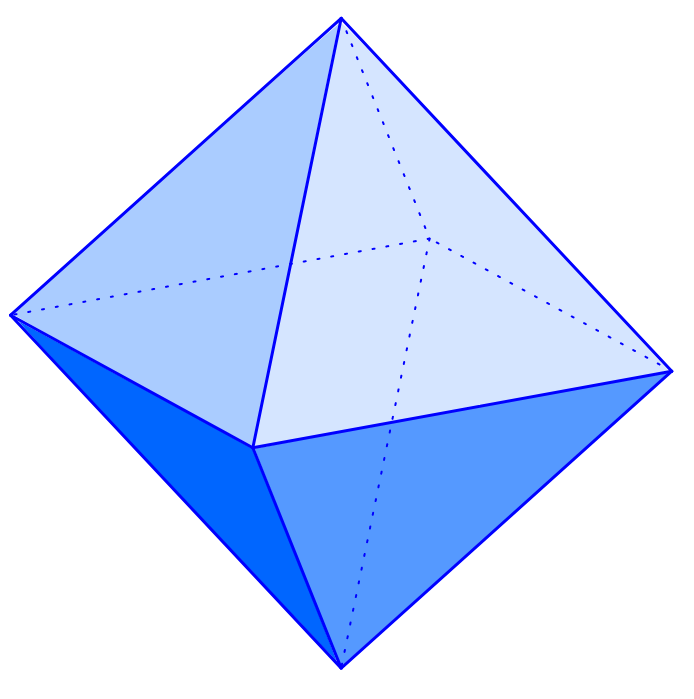
\includegraphics[width=0.7\linewidth]{figures/octahedron.png}
    \caption{Octahedron \protect\footnotemark}
    \label{fig:octahedron}
  \end{minipage}
  \begin{minipage}{0.5\textwidth}
    \centering
    \vspace{+0.8cm}
    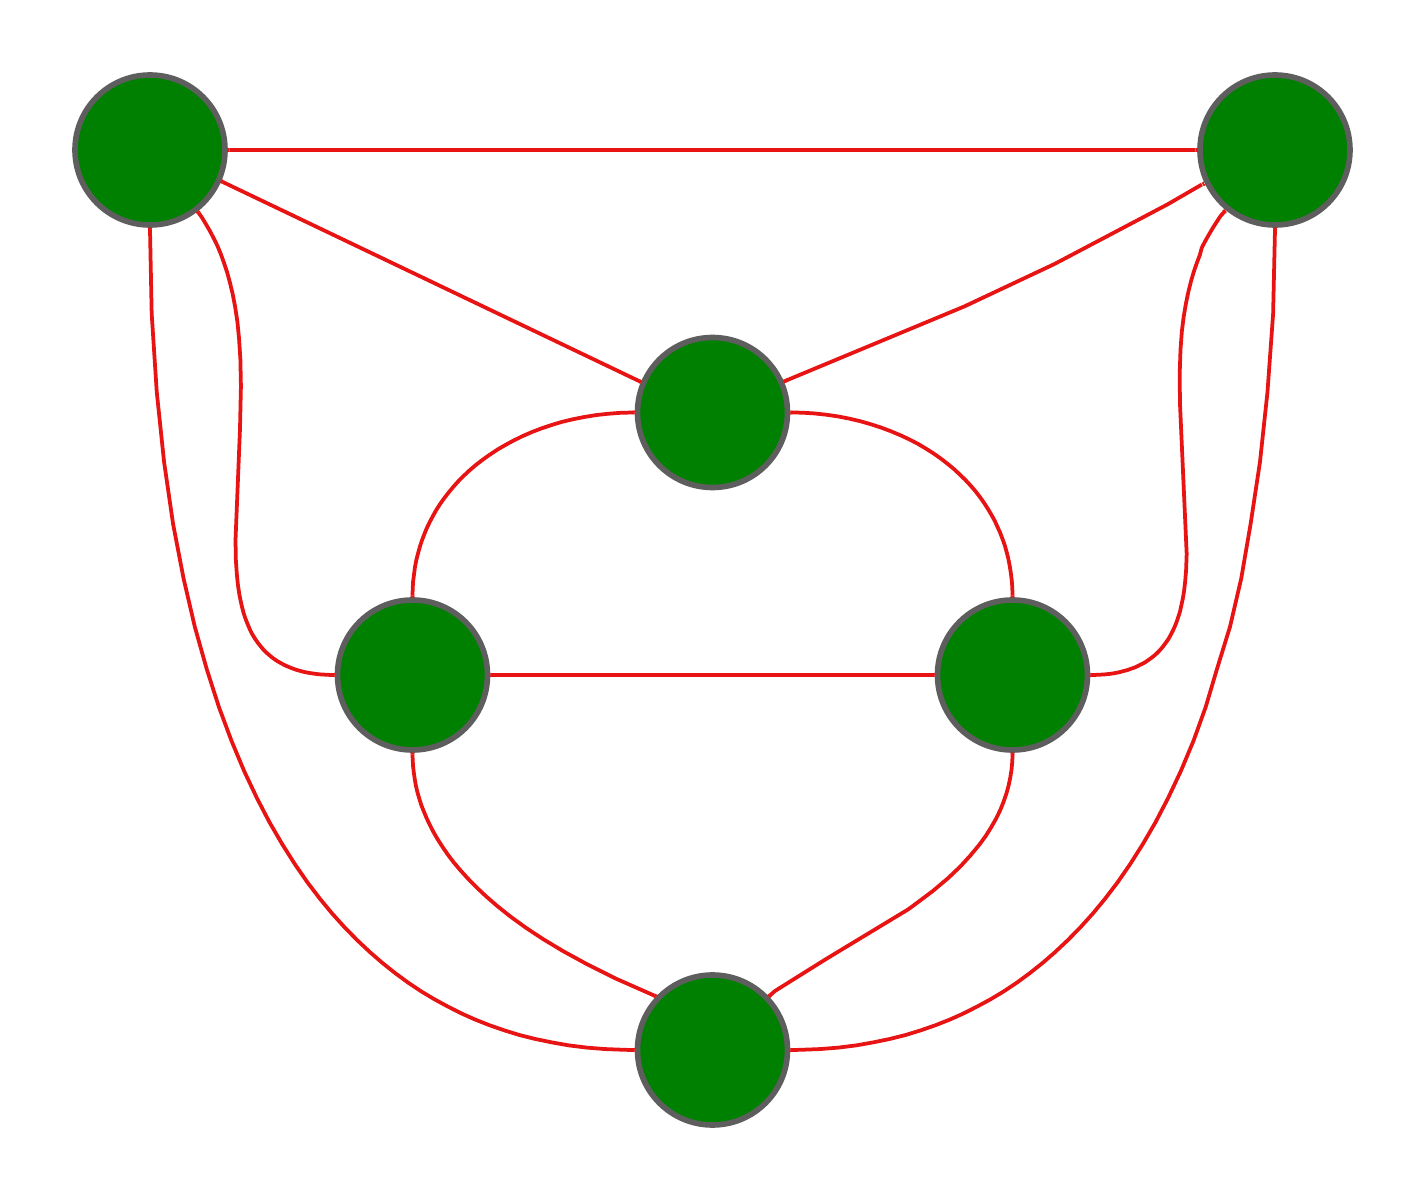
\includegraphics[width=0.7\textwidth]{figures/octahedron_graph.png}
    \caption{Octahedron Graph Interpretation}
    \label{fig:octahedron_graph}
  \end{minipage}
\end{figure}
\footnotetext{Rosemark, \textit{octahedron}, \url{https://cleanpng.com}, 30.11.2023}

%
%\begin{figure}[ht]
%    \centering
%    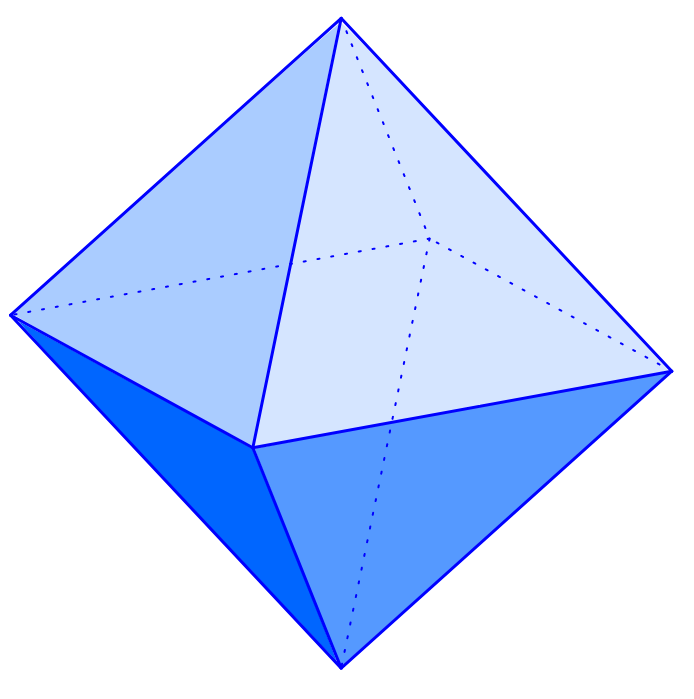
\includegraphics[width=0.5\linewidth]{figures/octahedron.png}
%    \caption{Octahedron \protect\footnotemark}
%    \label{fig:octahedron}
%\end{figure}
%
%\begin{figure}[ht]
%    \centering
%    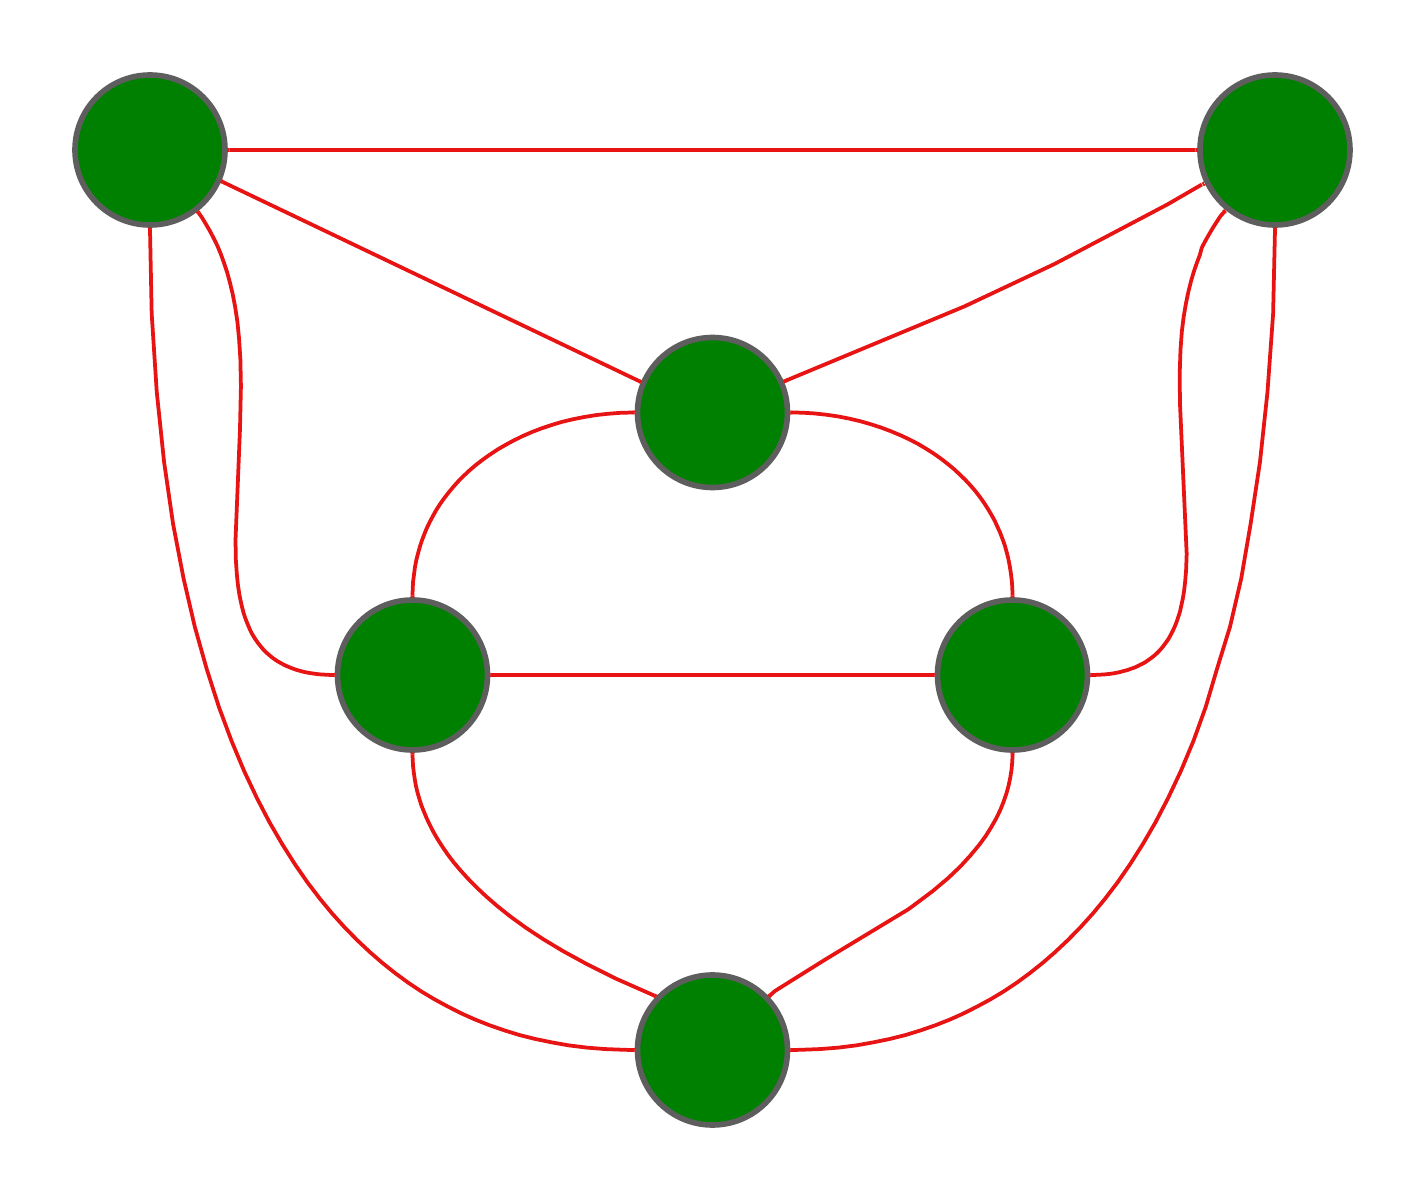
\includegraphics[width=0.525\textwidth]{figures/octahedron_graph.png}
%    \caption{Graph Interpretation of an Octahedron}
%    \label{fig:octahedron_graph}
%\end{figure}

\clearpage
\noindent
This graph can now be shown as a book embedding, in the form of a queue layout as well as using the track layout. The three visualizations shown in \cref{fig:octahedron_layouts} clearly highlight the differences between the layouts. While the book embedding divides the graph into distinct pages or layers to ensure non-crossing edges, the queue number layout organizes the edges into queues, aiming for a compact representation. It is noticeable that three tracks are required to represent the graph as a track layout. The other two alternatives just necessitate the use of two stacks, respectively, of queues to display the same graph.
\newline
In addition to other visualizations and an up-to-date collection\footnote{Sergey Pupyrev, \textit{Benchmark},\url{https://spupyrev.github.io/linearlayouts.html},  06.02.2024}
of existing results on stack and queue numbers, Pupyrev provides an existing tool to examine some layouts. The solver\footnote{Sergey Pupyrev, \textit{Solver},\url{http://be.cs.arizona.edu/}, 06.02.2024}
is SAT-based and can display graphs in stack or queue layouts, or a combination of the two.

\begin{figure}[ht]
    \centering
    \begin{subfigure}[b]{0.45\linewidth}
        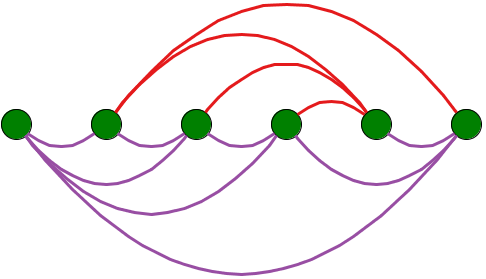
\includegraphics[width=\linewidth]{figures/octahedron_stack.png}
        \caption{Octahedron Graph drawn in 2 Stacks}
        \label{fig:octahedron_stack}
    \end{subfigure}
    \hfill 
    \begin{subfigure}[b]{0.45\linewidth}
        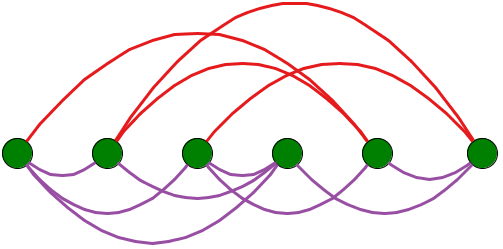
\includegraphics[width=\linewidth]{figures/octahedron_queue.png}
        \caption{Octahedron Graph drawn in 2 Queues}
        \label{fig:octahedron_queue}
    \end{subfigure}

    \begin{subfigure}[b]{0.45\linewidth}
        \centering
        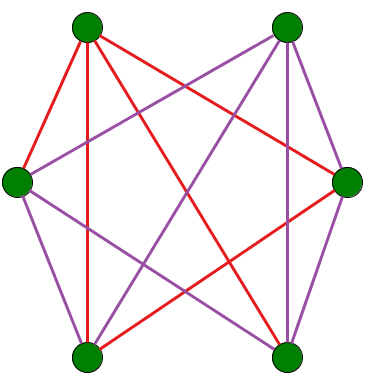
\includegraphics[width=0.8\linewidth]{figures/octahedron_tlp.png}
        \caption{Octahedron Graph drawn in 3 Tracks}
        \label{fig:octahedron_tlp}
    \end{subfigure}

    \caption{Octahedron Graph drawn in different Layouts³}
    \label{fig:octahedron_layouts}
\end{figure}

\clearpage

\section{Introduction to SAT-Solving}
Biere et al. \cite{Sat_solving} provide an excellent overview of the fields of logic and satisfiability. Based on this, we'd like to provide a brief introduction to the topic, which will serve as the foundation for the chapters that follow. 
\newline
Propositional logic has long been regarded as the foundation of reasoning in philosophy and mathematics. Its formalization as Boolean algebra was accompanied by the discovery that a large range of combinatorial problems can be represented as propositional satisfiability (SAT) problems. As a result, SAT solving became an important method in theoretical computer science and mathematical logic. It needs to solve SAT problems, which question whether it is possible to provide truth values to a Boolean formula in order for it to be evaluated as true. This topic is not simply of academic interest, but it also has significant practical relevance because it underpins various applications in cryptography, software verification, artificial intelligence, and optimization problems. Understanding the structure of those logical issues is critical to understanding the difficulty and utility of SAT solving. \newline
Conjunctive Normal Form (CNF) is commonly used to write SAT problems, in which a formula is an AND relation of many phrases and each clause is an OR relation of literals. A literal in this sense is a Boolean variable or its negation. Despite the fact that the structure's simplicity hides the potential complexity of the difficulties, its elegance allows for a consistent approach to problem solving. SAT solvers and sophisticated algorithms that use advanced methods like backtracking, unit propagation, and clause learning to answer these issues aid in the resolution of these problems. The evolution of these solvers throughout time is a monument to the inventiveness and perseverance of field researchers. Initially impossible issues are now frequently tackled, illustrating the extraordinary efficacy of these techniques. However, difficulties in SAT solving exist, particularly when dealing with extremely large or convoluted issues. \newline
The topic of SAT-solving research is dynamic and continuing, driven by the constant attempt to improve the efficiency of algorithms and heuristics. This search is not only intellectual; the ramifications in our world of complicated decision-making are far-reaching. Advances in SAT solving have the potential to uncover answers to some of the most difficult and convoluted issues in computer science and beyond.

\subsection{Complexity}
Within the field of computational computability, problem complexity is an essential aspect. Specifically, the classification of issues into several complexity classes and levels of difficulty. The study of NP-hard issues is a key component and a large area of research attention. These issues are well-known for being computationally challenging and are crucial to comprehending algorithms and their bounds.

\begin{definition}
    An \emph{NP-hard problem} refers to being at least as difficult as the most difficult problem in the NP complexity class. Any NP-hard problem in polynomial time can be reduced to any NP-hard problem in polynomial time. This means that if one NP-hard problem can be solved effectively (in polynomial time), then so can all NP problems.
\end{definition}
\noindent
The satisfiability problem of propositional logic also belongs to this class of problems. Furthermore, it has been proven to be NP-complete. Nevertheless, NP-hard problems are not necessarily in NP, i.e., they are not guaranteed to be verified in polynomial time. Because of its NP-hardness, the SAT serves as the foundation for classifying additional problems as NP-hard. If a problem can be reduced to SAT in polynomial time, it is also considered NP-hard \cite{SAT_Complexity}. \newline
When we look at the TLP through the lens of SAT, we get a boolean formula whose satisfiability determines whether there is a layout that follows the rules. This consideration will be important in our further experiments. If it is not immediately evident whether there are configurations that satisfy the formula or clauses that signal unfulfillability, all conceivable configurations must be checked in order to reach a solution. This could result in much longer processing times for larger variable sets.

\section{Related Work}
Looking at mathematical problems and general computer science problems from a SAT perspective is ubiquitous. Although graph problems are uncommon, they can still be solved using a propositional interpretation. The following work by Courcelle and Durand \cite{courcelle:hal-03668884} is an example of how SAT solvers can be used to solve graph problems. It primarily addresses the clique width, a graph parameter that describes a graph's structural complexity, and reduces it to a boolean satisfiability problem; it is closely related to tree width. The study discovered that previously established upper bounds for clique width are reachable. 
\newline
Another interesting work by Zhao et al. \cite{decomposing} systematically analyzes how problems related to decomposing graphs can be expressed as logic statements, allowing them to be solved using SAT-solver technology. By using methods to break symmetries, it is possible to solve previously unsolved cases and significantly reduce the computational time required to find decompositions. Nonetheless, some small instances continue to resist resolution, posing a compelling challenge to the capabilities of SAT-solver technology.
\newline 
A SAT-related approach has also been used in relation to layout problems.
In their paper "The Book Embedding Problem from a SAT-Solving Perspective", Bekos et al. \cite{book_embedding_sat} examined one of these graph problems. The researchers presented a simple and straightforward SAT formulation for graph queue number layout. They attempted to solve some non-trivial instances of this problem set in a reasonable amount of time using their SAT-formulation. Furthermore, various hypotheses about planar graphs were tested, and a lower bound of 4 for $b$ for 1-planar graphs was discovered. The following work is based on the methods and formulations shown by Bekos et al. and deals with the TLP in a similar way.

\chapter{SAT Formulations for the TLP} 
\label{chap:Formulation_of_tlp}
Let $G = (V,E)$ be the graph we consider in our problem, where $V =\{v_1,v_2,...,v_n\}$ represents the vertices and $E = \{e_1,e_2,...,e_n\}$ the corresponding edges of the graph. The primary objective is to determine whether there exists a Tracklayout $L$ for this graph that meets the conditions outlined in the previous section. To tackle this challenge, we first frame the problem in terms of a logical formula, denoted as $F(G, t)$. This formula seeks to address the problem by encoding it into a SAT instance. It's important to highlight that the formula is deemed satisfied if and only if there exists a layout $L$ that displays the initial graph $G$ on $t$ tracks. Our formula will hold the conjunctive normal form (CNF). The formula $F(G, t)$ is defined by its set of variables and the associated set of rules. The primary role of these rules is to ensure the correct assignment of the variables. They are expressed in a specific type of propositional logic, which can be transformed into CNF clauses straightforwardly \cite{conjunction}. In the following sections, we will define the variables we will need for our SAT formulation and examine various clause approaches that will help us comply with the ruleset.

\section{Variables and Clauses}
\label{sec:vars_clauses}
The purpose of this elaboration is to determine the most efficient SAT formulation for the TLP. Central to differentiating these formulations is their unique approach to representing crossings. This primarily involves specifying the positions of nodes on their respective tracks, a crucial aspect for identifying crossing edges. The competing SAT formulations have a similar basic structure, which we will define first before examining three different possibilities to identify and handle crossing edges.
\newline

%\subsection{Basic Variables and Clauses}
\label{sec:basic_clauses}

\noindent
The variables of $F(G, t)$ model a track layout of $G$ on $t$ tracks, if such a structure exists. To assign a node of the graph to a track, we use the variable $\sigma(v_i,t_k)$ for each pair of nodes $v_i \in V$ and track t. For instance, the assignment $\sigma(v_1, t_1)$ is considered true when node $v_1$ is positioned on track $t_1 \,$ in $\, L$. In order to formulate all possible assignments for each node on every track, a total of $ \vert V \vert \times t$ variables are required. We may now assign a track to each node using this variable. In order to fulfill the first rule of the TLP, uniqueness, we must verify that each node is on at most one track, which requires our first clauses. To maintain clarity, we will approach this in two parts, whereby the first one guarantees that every node is on at least one track:
    $$ (\sigma(v_i,t_1) \lor \sigma(v_i,t_2) \lor \dots \lor \sigma(v_i,t_n)) \, \forall v_i \in V \text{ and every track }t $$ 
Therefore, the first part of each of the clauses will contain $t$ variables. Next, we have to confirm that every node is on at most one track, which, combined with the first part, will ensure that for each node, precisely one of the track variables $\sigma$ evaluates to true, i.e., that each node is assigned to exactly one track. The second part is formulated as follows:
    $$ (\overline{\sigma(v_i, t_x) \land \sigma(v_i, t_y)}) \, \forall v_i \in V \text{ and every combination of two tracks } x, y \text{ with } x \neq y$$ 
\noindent
As outlined, we will ignore the diagonal of the track combinations. Also note that due to commutativity, $(\lnot \sigma(v_i, t_x) \lor \lnot \sigma(v_i, t_y))$ is the same as $(\lnot \sigma(v_i, t_y) \lor \lnot \sigma(v_i, t_x))$. This assumption helps us to reduce the number of variables by a significant amount and thus obtain a total number of $\frac{(\vert V \vert^2-\vert V \vert)}{2}$ disjunctions of two negated literals, each resulting in $2 \times \frac{(\vert V \vert^2-\vert V \vert)}{2}$ variables for the second part of this rule. All in all, when we merge these two parts, we need $\vert V \vert$ larger clauses with $t + 2 \times \frac{(\vert V \vert^2-\vert V \vert)}{2}$ variables each to establish the first rule. The next clauses enforce that neighboring nodes are on the same track and require us to include the edges of the graph in our formulation. This can be achieved by adding the following conjunctions:
        $$ \forall e_{i,j} \in E : (\overline{\sigma(v_i,t_x) \land \sigma(v_j,t_x)}) \text{ for every track } t $$ 
This phrasing leads to a total of $\vert E \vert \times t$ clauses with one negated conjunction each, or more precisely, $2 \times (\vert E \vert \times t)$ variables per clause. With the help of the clauses defined so far, we can now assign a unique track to each node without breaking the rules of the TLP. 

\subsection{First Approach on Crossing Edges}
Now we turn our attention to the core problem of the track layout, namely the restriction of forbidden crossings. To detect crossings in the layout, we first need a way to determine the position of the nodes within the tracks. The simplest way to arrange the nodes would be to include a variable that assigns each node a unique number that indicates its position along the tracks. Therefore, we define the tuple $\phi(v_i,p)$ for each $v_i \in V$ and $p$ up to the total number of nodes. Hence $\phi(v_i,p)$ is true when $v_i$ is in position $p$. Note that the nodes are taken in a total order, so we can assume that for each node $v$ exactly one variable $\phi(v_i,p)$ must be true. Ultimately, this method results in ${\vert V \vert}^2$ variables to express all possible orders. Furthermore, clauses would be required to ensure that no two nodes are in the same position. This specification works equivalent to rule 1 and results in $\vert V \vert$ clauses with $\vert V \vert + 2 \times \frac{(\vert V \vert^2-\vert V \vert)}{2}$ variables. To better understand this definition, let's take a look at the \cref{fig:order_example_tot} below.

\begin{figure}[ht]
  \centering
  \begin{minipage}{0.6\textwidth}
    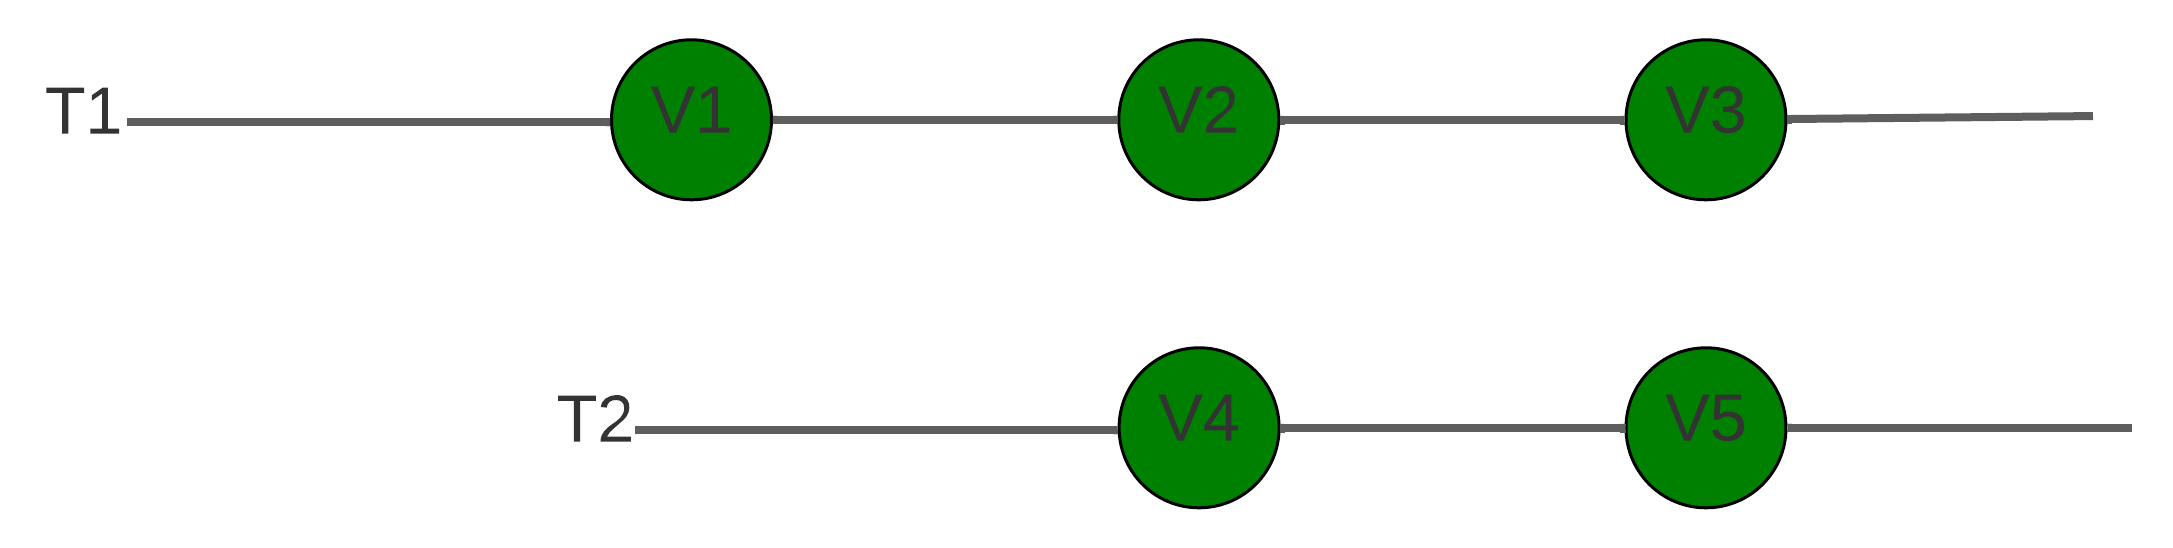
\includegraphics[width=\linewidth]{figures/Order_example.png} 
  \caption{Example for Total Ordering}
  \label{fig:order_example_tot}
  \end{minipage}%
  \begin{minipage}{0.4\textwidth}
    To formulate this sequence of nodes, these variables must come true:
    \begin{itemize}
    \item  $\phi(v_1,1)$, $\phi(v_2,2)$, $\phi(v_3,3)$, $\phi(v_4,4)$ and $\phi(v_5,5)$
    \end{itemize}
  \end{minipage}
\end{figure}
\noindent
It is critical to remember that $\phi$ alone is insufficient to define a distinct sequence, as it does not provide any information about the tracks on which the nodes are distributed. To correctly formalize the preceding example, the following five variables must also be set to true: 
$$\sigma(v_1, t_1), \sigma(v_2, t_1), \sigma(v_3, t_1), \sigma(v_4, t_2) \text{ and } \sigma(v_5, t_2)$$
\noindent
Next, we must exclude all possibilities of forbidden crossings. To accomplish this, we create the following formula using $\phi$ and $\sigma$:
    $$ \forall e_{i,j}, e_{u,w} \in E, \ \forall m,n,a,b \text{ in range of } \vert V \vert \text{ with } m<n, \, a<b:$$
    $$(\overline{\sigma(v_i,t_x) \land \sigma(v_u,t_x) \land \sigma(v_j,t_y) \land \sigma(v_w,t_y) \land \phi(v_i,p_m) \land \phi(v_u,p_n) \land}$$
    $$ \overline{\phi(v_w,p_a) \land \phi(v_j,p_b)})\text{ for all disjoint pair of tracks } t_x \text{ and } t_y $$
To have a better understanding of this rather larger formula, we shall analyze it in further detail. Since we are considering edge pairs, we need $\vert E \vert^2$ clauses. Logically, we do not consider self-edges, or in other words, non-disjoint edge pairs, and get a total of $(\vert E \vert^2 - \vert E \vert)$ as our first factor. In addition, there will be another one for the disjoint track pairs. As commutativity also works in our favor here, we only have to care about one of the pairs $(t_x, t_y)$ and $(t_y, t_x)$. The corresponding alternative can already be covered while calculating the clauses for the first one. Adding $\frac{(t^2-t)}{2}$ clauses for the tracks, the only thing missing is the inclusion of the appropriate positions. We first choose two positions for $m$ and $n$. Let these be distinct, but fixed. Since we operate on a total order, each position may only occur once. Therefore, we know that the number of remaining positions for $a$ and $b$ must be two less. Summarized for this interpretation, we gain a total of 
$ (\vert E \vert^2 - \vert E \vert)) \times \frac{(t^2-t)}{2} \times \frac{(\vert V \vert^2-\vert V \vert)}{2} \times \frac{((\vert V \vert-2)^2-(\vert V \vert-2))}{2}$ clauses.
\noindent \newline
At first glance, the problem seems to have been solved. However, the positioning of the nodes among the individual tracks seems to cause a problem, as we have not yet introduced any restrictions for the track transitions. The distribution within a track also poses a similar kind of problem with this formulation. The first approach appears to be missing conditions to create a unique variable assignment. Looking at the example in \cref{fig:order_example_tot}, $\phi$ appears to be a valid method of storing the vertexes order. On the other hand, just designating the position variables does not guarantee that the nodes in $T$ are consecutively numbered. In our illustration, $\phi(v_2,2)$ and $\phi(v_3,3)$ are set to true, but $\phi$ itself is not fixed according to the current definition and would therefore have to be interpreted individually for each pair of nodes. For this reason, it has not yet been assured that node $v_2$ is located to the left of node $v_3$.
The same applies to all other node pairs for each track. In order to maintain a clear position of the nodes in relation to each other, we need to introduce rules to prevent certain configurations. \newline
One way to define the exact position in $L$ would be to force a node $v_i$ with $\sigma(v_i,t_1)$ to the first position with the help of further clauses, and to force another node $v_j$ with $\sigma(v_j,t_{max})$ to the last position. This should be repeated until you have a correct setup by setting nodes to the second and second last position, the third and third last positions, etc. Another alternative would be to look at the relationship between nodes. To do this, for each node $v_i$ and $\sigma(v_i, t_y)$, state that all other nodes $v_j$ with $\sigma(v_j, t_x)$ and $t_x < t_y$ have a position that is smaller than the position of $v_i$ and have a greater position than $v_i$ if $t_x > t_y$. However, this idea appears to require an excessive amount of effort and would increase the number of clauses considerably because it only limits the problematic areas we have using this method. As the approach of structuring the nodes on the basis of a single total order does not seem suitable, we will not consider it further for the time being.
\subsection{Second Approach on Crossing Edges}
\label{sec:approach2}
To more precisely specify the order, we require variables that allow us to view and compare the neighboring nodes for each node in L. We can also prohibit crossings if we have access to all nodes and their neighbors on the respective tracks. As a result, we are now taking a different approach and defining a new variable $\omega$ to determine the relationship between two nodes. We define this variant as the tuple $\omega(v_i,v_j)$ for each $v_i,v_j \in V$. This variable evaluates to true if $v_i$ is one of the left neighbors of $v_j$ on any track. Notice that variables $\omega(v_i,v_j)$ with $i = j$ cannot be evaluated as true because this will refer to $v_i$ and $v_j$ being the same node, which obviously cannot be the left neighbor of itself. This will eventually lead to ${\vert V \vert}^2$ variables. In this relative encoding of the sequence between nodes, clearly, asymmetry has to hold for these variables, which will be ensured by the following rule: 
    $$ \omega(v_i,v_j) \leftrightarrow \lnot \omega(v_j,v_i) $$ 
To reduce the total set of clauses by a substantial sum, we define the asymmetry of the variable $\omega(v_i,v_j)$ only for the case that $i < j$. The other literals $\omega(v_i,v_j)$ with $i > j$ can be replaced with the respective counterpart $\lnot \omega(v_j,v_i)$, leading to $\frac{(\vert V \vert^2-\vert V \vert)}{2}$ clauses \cite{asymmetric}. In order to establish a proper order within a track, we must also ensure transitivity with total ${\vert V \vert}^3$ clauses. This is done as follows:
    $$ \omega(v_i,v_j) \land \omega(v_j,v_k) \rightarrow \omega(v_i,v_k) \, \forall \text{ pairwise distinct } v_i,v_j,v_k \in V$$ 
Additionally, we implement $t \times {\vert V \vert}^2$ clauses, which cause that a node can only lie to the left of another node if both nodes are positioned on the same track. If this requirement did not exist, there would be considerable difficulties with the track breaks of the eventual node positioning:
    $$ \omega(v_i,v_j) \rightarrow \sigma(v_i,t_k) \land \sigma(v_j,t_k) \, \forall \text{ pairwise distinct } v_i,v_j \in V \text{and every track }t$$ 
Therefore, it is important to note that there are indeed nodes $v_i$ for which none of the variables $\omega$ with $\omega(v_i,v_n) \forall v_n \in V$ evaluates to true. This is precisely the case when the node n is on the right edge of the track. We will again point out this method with the help of the same example in \cref{fig:order_example_rel} we looked at before to truly understand the definition of this order implementation. 

\begin{figure}[ht]
  \centering
  \begin{minipage}{0.6\textwidth}
    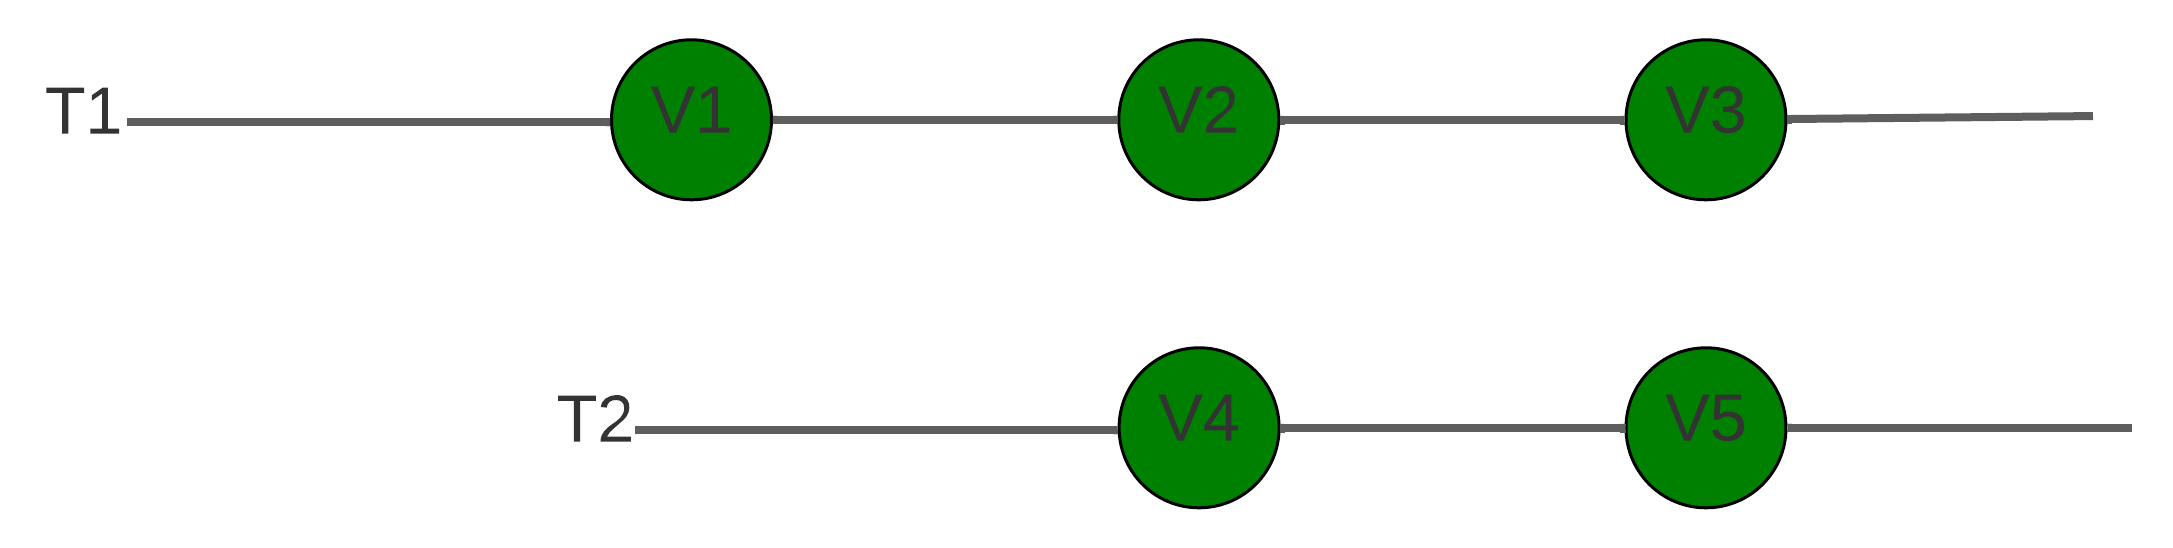
\includegraphics[width=\linewidth]{figures/Order_example.png} 
  \caption{Example for Relational Ordering}
  \label{fig:order_example_rel}
  \end{minipage}%
  \begin{minipage}{0.4\textwidth}
    To formulate this sequence with the relational method, these variables must come true:
    \begin{itemize}
    \item  $\omega(v_1,v_2)$, $\omega(v_1,v_3)$, $\omega(v_2,v_3)$ and $\omega(v_4,v_5)$
    \end{itemize}
  \end{minipage}
\end{figure}
\noindent
\newline
\newline
Remember that $\omega$ alone is not enough to provide the complete track layout. Next, we have to block the intersections of edges using our new approach. This can be reached with the following conjunctions, which we build for each disjoint pair of edges $e_{i,j}, e_{u,w}$ so that:
    $$ \forall e_{i,j}, e_{u,w} \in E : \overline{(\sigma(v_i,t_x) \land \sigma(v_u,t_x) \land (\sigma(v_j,t_y) \land (\sigma(v_w,t_y) \land}$$ 
    $$ \overline{\omega(v_i,v_u) \land \omega(v_w,v_j)}\text{ for all disjoint pair of tracks } t_x \text{ and } t_y $$
Using this method, we can cut out a whole factor that was used to define the positions in the total order. We don't need to manifest the position of the nodes in an own variable since we can also extract a unique order from only the relations between each node. At the end, this results in 
$ (\vert E \vert^2 - \vert E \vert)) \times \frac{(t^2-t)}{2}$ clauses with 6 negated variables each.

\subsection{Third Approach on Crossing Edges}
\label{sec:approach2_2}
In general, there are numerous ways to improve SAT formulas. In our third attempt, we reduced the number of clauses as well as their size. We use the same foundation as in the second approach. Looking at the previous formula, it is interesting to note that we used an entire loop to handle the track pairs. The next consideration is what possibilities there are to reduce this factor. \newline
One idea for looking beyond this loop is to define a new variable that indicates that two nodes are on the same track. According to this formula, it doesn't matter which track the nodes are on, as long as they're on the same one. We therefore define a new variable $\psi$ for which $\psi(v_i,v_j) \forall v_i,v_j \in V$ evaluates to true if and only if $v_i$ and $v_j$ are on the same track. With the introduction of a new variable, we are obviously increasing the general handling of our phrases while needing ${\vert V \vert}^2$ variables for every possibility of every two nodes being on the same track. To apply this variable correctly, we need additional clauses that enforce our interpretation of $\psi$. Similar to the implication for the correctness of $\omega$ formulated in the second approach, we need $t \times {\vert V \vert}^2$ clauses, which are worded as follows:
    $$ \sigma(v_i,t_k) \land \sigma(v_j,t_k)\rightarrow \psi(v_i,v_j) \, \forall v_i,v_j \in V \text{and every track }t$$ 
With the help of this new variable, it is possible to limit the crossing clauses. Again, we have to formulate a conjunction that we construct for every disjoint pair of edges $e_{i,j} e_{u,w}$ in order to:
    $$ \forall e_{i,j}, e_{u,w} \in E : \overline{(\psi(v_i,v_u) \land \psi(v_j,v_w) \land   \omega(v_i,v_u) \land \omega(v_w,v_j)}$$ 
This formulation allows us to ignore another factor in our quantity of clauses and so on decrease the required clauses to $ (\vert E \vert^2 - \vert E \vert))$ and reduce the variables per clause by two. It is important to note that we indeed reduced the clause size of the most important rule. On the other hand, this approach requires an additional variable and an extra clause to properly introduce this variable. The later evaluation will show whether the reduction in the number of clauses is sufficient to be the significantly better method.

\section{Hypotheses}
Since we have now addressed three SAT formulations, we can begin to make some considerations and expectations for the upcoming evaluation of each of these methods. We will exclude the first formulation from the testing because we rated it significantly worse at an early stage and thus had not fully developed it. Instead, we will look at the second and third versions of our SAT formulations. As a result, we will compare their quality and place an emphasis on various aspects such as clause set size, evaluation, and creation time. So, before we describe our test data, we hypothesize the following:

\begin{enumerate}
    \item[H1:] The third method significantly reduces the number of clauses in the formulation, regardless of the fact that it includes an additional variable and associated clauses.
    \item[H2:] Despite having more variables, the formula created by the third approach will take significantly less time to evaluate, depending on the number of clauses.
\end{enumerate}


\chapter{Implementation and Test-cases}
Even though Python does not offer the same performance as lower-level programming languages (such as C/C++), we opt for it to implement the TLP and its solution approaches. Python has certain benefits, like readability and flexibility, which are helpful for the nested loops that make up the clauses. Furthermore, we have easy access to Sat-Solvers through the variety of libraries, which we can use to create, modify, and solve our formula.

\section{Introduction to the Python-SAT Library}
PySAT\footnote{\url{https://pysathq.github.io/}} is a Python library for editing, solving, and analyzing Boolean formulas and SAT (satisfiability) problems \cite{PySAT}. Born out of the need to create a unified and efficient collection of tools for SAT-related tasks in Python, PySAT integrates a number of widely used state-of-the-art SAT solvers such as MiniSat\footnote{\url{http://minisat.se/}}, Glucose\footnote{\url{https://www.labri.fr/perso/lsimon/research/glucose/}} and Lingeling\footnote{\url{https://fmv.jku.at/lingeling/}}. The library allows users to efficiently formulate Boolean formulas and analyze solutions, making it a valuable tool in research and development. Overall, PySAT provides an efficient and flexible platform for working on a wide range of Boolean logic and optimization problems. Its ease of use and performance make it a popular choice for many scientific and industrial applications. \newline
Among the numerous core modules of the PySAT toolkit, we will mainly use formula and solver. While solvers are Python wrappers for the code originally implemented in the C/C++ languages, the formula module is a pure Python module. Boolean variables in PySAT are represented using natural numbers, with $\mathbb{N}^+\setminus\{0\}$. According to this representation, a literal is an integer, with $-1$ representing the literal $\lnot x_1$ and $5$ representing the literal $x_5$. Moreover, a clause refers to a set of literals, with $[-3, -2]$ being an example of the clause $(\lnot x_3 \lor \lnot x_2)$ \cite{PySAT}. After variables and clauses are created, they can easily be added to a formula, which can be solved by any solver contained in the library. The important thing here is that the formulas that the solver requires for evaluation are always converted into a CNF. The \texttt{solve()} method returns an assignment of the variables if the formula has a solution, or a false if the solution set is empty. \newline
To evaluate the formulas for solving the TLP in the following, we use the SAT solver Lingeling. Lingeling is a fork of the PrecoSAT\footnote{\url{https://fmv.jku.at/precosat/}} prototype. Its data structures are designed to take up much less space. Large clauses with four or more literals, for example, are stored separately on literal stacks \cite{LingeLing}. In our scenario, we'll test the final two alternatives in the same way. In the first stage, we must build the variables and clauses required to explicitly define our problem. We now use PySAT to compose a larger logical statement, which Lingeling will analyze in the final and actual calculation step. As stated in \cref{chap:Formulation_of_tlp}, our goal is to complete $F(G,t)$. In order to gain a layout that uses as few tracks as possible, we loop through track numbers, starting with one track. If $F$ is evaluated as false, there is no viable configuration of our formula and therefore no track layout for $G$ with $t$ tracks. In this case, we increment $t$ until $F(G,t)$ is true. 

\section{Scenario and Environment}
The various tests were carried out using a machine with the characteristics shown in the specification \cref{tab:specs}.

\begin{table}[h]
\centering
\begin{tabular}{|l|l|}
\hline
\textbf{Component}      & \textbf{Specification} \\ \hline
Processor       & Intel i5-8250U @ 3.400GHz      \\ \hline
Memory          & 8 GB LPDDR4X RAM               \\ \hline
Storage         & 512 GB SSD                     \\ \hline
Operating System & Linux Mint 21.1 x86\_64        \\ \hline
Programming Language & Python 3.10.0       \\ \hline
\end{tabular}
\caption{Specifications of Acer Swift 5}
\label{tab:specs}
\end{table}

\subsection{Dataset}
Since the utilization of robust and diverse datasets is a crucial point for the advancement of algorithmic research, we decided to get our data from a well-known graph layout benchmark datasets\footnote{\url{https://visdunneright.github.io/gd_benchmark_sets/}} \cite{Benchmark}. The accessed source contains a list of benchmark datasets for testing graph layout algorithms, whereby the collection was originally summarized and is maintained by the \textit{Northeastern University Visualization Lab}. Therefore, we decided to use the \textbf{Rome-Lib} dataset that was collected by Di Battista et al\text{.} and first introduced in their paper \glqq An experimental comparison of four graph drawing algorithms\grqq \, in 1995 \cite{Rome_Lib}. 
\newline
Using this dataset, which provides a wide array of diverse graphs all within a range of $10$ to $100$ nodes, we chose $100$ undirected graphs in total to evaluate our algorithms. In order to cover the widest possible variety of cases and graph sizes, the set of test graphs contained $10$ graphs with $10\times n$ nodes each. More precisely, 10 graphs with 10 nodes each, 10 graphs with 20 nodes each, etc. To ensure a neutral selection of graphs without pre-filtering for characteristics, the 100 test data were randomly selected and retained using a small Python script. The individual test graphs and their rough properties are listed in the \cref{tab:Test_Data} on the next page.
\newline


\newpage

\begin{minipage}{.32\textwidth} % Erste Tabelle
\hspace*{-2.1cm} 
\vspace*{0.75cm}
\begin{tabular}{|c|c|c|}
\hline
Name & Nodes & Edges \\
\hline
grafo1972 & 10 & 15 \\
grafo1098 & 10 & 9 \\
grafo327 & 10 & 10 \\
grafo898 & 10 & 9 \\
grafo210 & 10 & 10 \\
grafo460 & 10 & 9 \\
grafo949 & 10 & 10 \\
grafo1627 & 10 & 15 \\
grafo2538 & 10 & 10 \\
grafo254 & 10 & 11 \\
\hline
grafo270 & 20 & 30 \\
grafo3051 & 20 & 23 \\
grafo413 & 20 & 24 \\
grafo1024 & 20 & 21 \\
grafo2922 & 20 & 24 \\
grafo1837 & 20 & 24 \\
grafo1716 & 20 & 23 \\
grafo2396 & 20 & 24 \\
grafo1901 & 20 & 26 \\
grafo874 & 20 & 25 \\
\hline
grafo176 & 30 & 35 \\
grafo358 & 30 & 39 \\
grafo1246 & 30 & 36 \\
grafo1334 & 30 & 39 \\
grafo484 & 30 & 35 \\
grafo1627 & 30 & 40 \\
grafo1687 & 30 & 32 \\
grafo1623 & 30 & 41 \\
grafo4040 & 30 & 36 \\
grafo1958 & 30 & 33 \\
\hline
grafo7330 & 40 & 50 \\
grafo7000 & 40 & 50 \\
grafo10615 & 40 & 50 \\
grafo7121 & 40 & 50 \\
grafo5675 & 40 & 44 \\
grafo10402 & 40 & 47 \\
grafo3335 & 40 & 53 \\
grafo6115 & 40 & 46 \\
grafo9997 & 40 & 50 \\
grafo5772 & 40 & 49 \\
\hline
\end{tabular}
\end{minipage}%
\hfill 
\begin{minipage}{.32\textwidth} % Zweite Tabelle
\hspace*{-0.5cm} 
\begin{tabular}{|c|c|c|}
\hline
Name & Nodes & Edges \\
\hline
grafo3744 & 50 & 72 \\
grafo4603 & 50 & 69 \\
grafo6775 & 50 & 63 \\
grafo6838 & 50 & 60 \\
grafo4945 & 50 & 69 \\
grafo1528 & 50 & 56 \\
grafo3780 & 50 & 63 \\
grafo3685 & 50 & 72 \\
grafo6740 & 50 & 66 \\
grafo6264 & 50 & 72 \\
\hline
grafo4620 & 60 & 75 \\
grafo9484 & 60 & 78 \\
grafo6483 & 60 & 83 \\
grafo1192 & 60 & 79 \\
grafo5896 & 60 & 84 \\
grafo8586 & 60 & 79 \\
grafo4436 & 60 & 78 \\
grafo7448 & 60 & 81 \\
grafo5483 & 60 & 75 \\
grafo4376 & 60 & 73 \\
\hline
grafo1381 & 70 & 87 \\
grafo9300 & 70 & 96 \\
grafo8237 & 70 & 98 \\
grafo7992 & 70 & 94 \\
grafo9739 & 70 & 85 \\
grafo8105 & 70 & 100 \\
grafo8187 & 70 & 89 \\
grafo4558 & 70 & 92 \\
grafo9297 & 70 & 96 \\
grafo9569 & 70 & 91 \\
\hline
grafo9582 & 80 & 101 \\
grafo5370 & 80 & 111 \\
grafo4865 & 80 & 117 \\
grafo9096 & 80 & 108 \\
grafo9797 & 80 & 107 \\
grafo4890 & 80 & 108 \\
grafo9795 & 80 & 117 \\
grafo7907 & 80 & 127 \\
grafo8058 & 80 & 111 \\
grafo5558 & 80 & 108 \\
\hline
\end{tabular}
\captionof{table}{100 Test Graphs}
\label{tab:Test_Data}
\end{minipage}%
\hfill 
\begin{minipage}{.32\textwidth} % Dritte Tabelle
\hspace*{1cm} 
\vspace*{10.35cm}
\begin{tabular}{|c|c|c|}
\hline
Name & Nodes & Edges \\
\hline
grafo8959 & 90 & 121 \\
grafo8840 & 90 & 117 \\
grafo8494 & 90 & 119 \\
grafo7130 & 90 & 125 \\
grafo8558 & 90 & 125 \\
grafo8952 & 90 & 128 \\
grafo8756 & 90 & 117 \\
grafo8946 & 90 & 125 \\
grafo8711 & 90 & 121 \\
grafo3756 & 90 & 127 \\
\hline
grafo8793 & 100 & 138 \\
grafo10633 & 100 & 138 \\
grafo10820 & 100 & 141 \\
grafo10750 & 100 & 135 \\
grafo8674 & 100 & 135 \\
grafo10153 & 100 & 136 \\
grafo10644 & 100 & 145 \\
grafo10603 & 100 & 136 \\
grafo10998 & 100 & 142 \\
grafo10257 & 100 & 124 \\
\hline
\end{tabular}
\end{minipage}

\newpage

\chapter{Results}
This section presents the results of our experimental study on the TLP. To effectively analyze the performance and characteristics of the proposed algorithms, we used two types of graphical representations: box plots and line graphs. Box plots were used to compare the time efficiency of the two algorithms. They excel at displaying data distributions, highlighting median values, and identifying outliers. This method allows for an immediate visual comparison of the methods, providing insights into their performance in terms of speed across different test cases. To learn more about the approaches' internal mechanics, we created line graphs focusing on the number and relevance of clause sets in different SAT formulations. Line graphs are excellent for depicting trends and changes over a series of data points. In this context, they provide a clear visual representation of how the number and significance of clause sets change as the graph's complexity increases. 
\section{Test Outcomes}
\Cref{fig:clause_growth} below provides a visual representation of the relationship between graph complexity, as measured by node count, and the subsequent growth of clauses in the two distinct SAT solving approaches. As the graph's size increases, so does the number of clauses for both methodologies. This upward trend is strong and consistent, indicating a direct relationship between graph intricacy and clause volume. Notably, the second approach consistently generates more clauses than the third, across the range of node counts tested, with the exception of the smallest graphs. This method results in an average of nearly 6 million clauses for the largest graphs tested, which exceeds its counterpart by approximately 1 million clauses.
\begin{figure}[ht]
    \hspace{-1,75cm}
    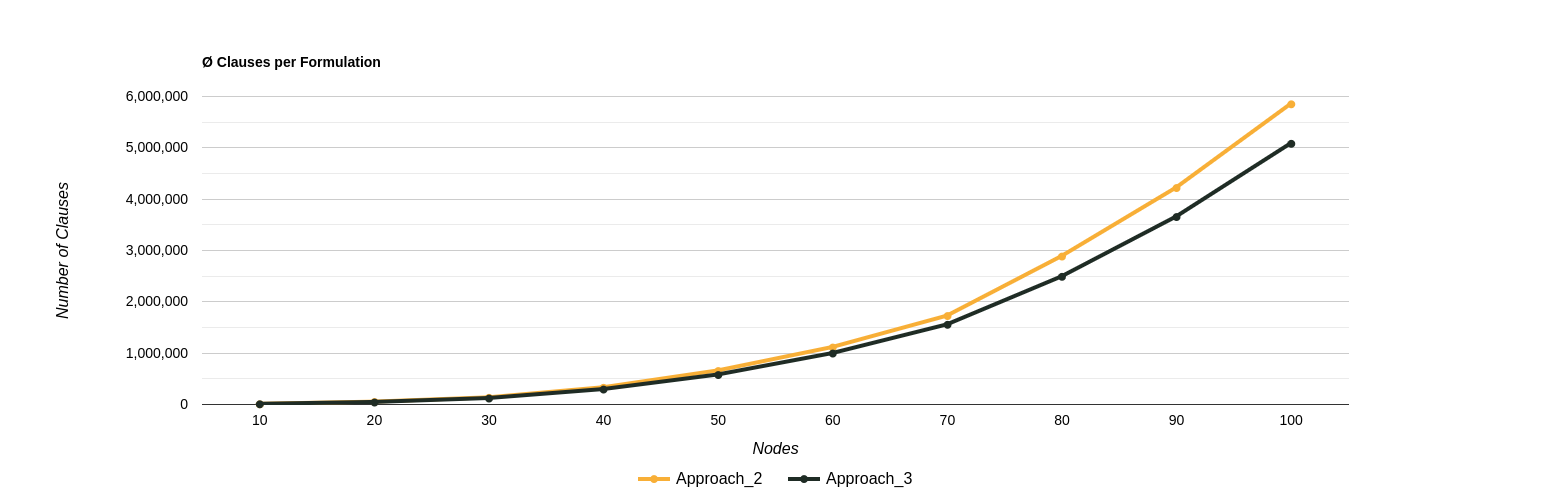
\includegraphics[width=1.3\textwidth, height=0.23\textheight]{figures/Clause_Growth_with_Nodes.png}
    \caption{Clause Growth with increasing Nodes}
    \label{fig:clause_growth}
\end{figure}

\noindent
Generally, our tests involve two steps: initially, our algorithms create SAT formulations, followed by the solver to evaluate those phrases. The proportional distribution of the calculation steps is considered a critical factor in assessing the performance and efficiency of SAT-solving methodologies. Consequently, the charts now shown delineate this distribution of computing time, dividing it between clause creation and clause evaluation.
\begin{enumerate}
    \item [Fig. 5.2:] For graphs with 10 to 60 nodes, the chart reveals that the majority of computing time is devoted to the creation of clauses. Notably, there's a dramatic shift observed when handling graphs with 70 or more nodes. The computing time ratio inverts, with clause evaluation now consuming almost 100\%.
    \item [Fig. 5.3:] A similar pattern emerges, yet the transition appears more gradual. The clause creation process initially consumes a larger time percentage, which then gradually cedes to clause evaluation as the dominant time consumer. Interestingly, the trend briefly reverses near the 50-node benchmark, where the time spent on clause evaluation momentarily spikes to 57\%.
\end{enumerate}

\begin{figure}[ht]
    \hspace{-0.9cm}
    \includegraphics[width=1.1\textwidth, height=0.3\textheight, keepaspectratio]{figures/Of_Calculation_Time_Approach_3.png}
    \caption{Percentage Calculation Spread Appraoch 3}
    \label{fig:Percentage_3}
\end{figure}

\begin{figure}[ht]
    \hspace{-0.9cm}
    \includegraphics[width=1.1\textwidth, height=0.3\textheight, keepaspectratio]{figures/Of_Calculation_Time_Approach_2.png}
    \caption{Percentage Calculation Spread Appraoch 2}
    \label{fig:Percentage_2}
\end{figure}

\noindent
The subsequent series of diagrams offers a comprehensive comparison of the total calculation times associated with two distinct approaches to solving the track layout problem. In addition to the attempts at finding a solution, the times of the calculation when no valid track layout for the graph was found are taken into consideration as well. The box plots all have the same structure: the two variants are distributed on the y-axis, while the calculation time is located in different sizes on the x-axis.

\begin{figure}[ht]
  \centering
  \begin{minipage}{0.5\textwidth}
        \hspace{-1cm}
        \includesvg[width=1.2\linewidth]{figures/Box_Plot_10_Nodes_1.svg}
  \caption{10-Node-Graph Calculation}
  \label{fig:Calc_10_Nodes}
  \end{minipage}%
  \begin{minipage}{0.5\textwidth}
  \vspace{-0.3cm}
    \Cref{fig:Calc_10_Nodes} shows a box plot designed to analyze the calculation times of graphs with ten nodes each. The third approach has a median calculation time of around one millisecond, which is slightly faster than the second approach. Despite this, the second approach has slightly more variation in its calculation times. We find that the two approaches' outliers are the most intriguing aspect. These don't necessarily have to impact the same graphs, like in this instance.
  \end{minipage}
\end{figure}
\noindent
Notably, the second one contains outliers, with the most extreme examples being graph instances \textit{grafo1627} and \textit{grafo1972}, which measure in at 6 milliseconds and 5 milliseconds, respectively. In contrast, the third version shows a tighter cluster of data points, approaching the 2-millisecond threshold with only one outlier. Surprisingly, both methods struggled with the graph \textit{grafo1972}, but the third approach was able to compute a solution more than twice as quickly. Moving on to the analysis of graphs with 20 nodes.
\noindent
\begin{figure}[ht]
  \centering
  \begin{minipage}{0.5\textwidth}
        \hspace{-0.9cm}
        \includesvg[width=1.2\linewidth]{figures/Box_Plot_20_Nodes_1.svg}
  \caption{20-Node-Graph Calculation}
  \label{fig:Calc_20_Nodes}
  \end{minipage}
  \begin{minipage}{0.47\textwidth}
  \vspace{-0.3cm}
In \cref{fig:Calc_20_Nodes}, we see consistency in median calculation times, with the second approach averaging around 15 milliseconds and the alternative method counting about 12 milliseconds. The third approach's variance approaches 60 milliseconds, in contrast to the second method, which does not exceed 40 milliseconds. Outliers occur across each method, with approach two exhibiting two notable deviations and the third presenting one fewer. 
  \end{minipage}
\end{figure}
\\
These outliers are indicated by calculation times of 100 and 159 milliseconds for the graphs \textit{grafo1716} and \textit{grafo413}. Once again, both methods faced the same challenge with the graph \textit{grafo413}, where the third approach took significantly longer, nearly 330 milliseconds, to resolve the correct layout.

\begin{figure}[ht]
  \centering
  \begin{minipage}{0.5\textwidth}
        \hspace{-1.3cm}
        \includegraphics[width=1.25\linewidth]{figures/Box_Plot_30_Nodes_1.pdf} 
  \caption{30-Node-Graph Calculation}
  \label{fig:Calc_30_Nodes}
  \end{minipage}%
  \begin{minipage}{0.45\textwidth}
  \vspace{-1cm}
  For graphs with 30 nodes, as shown in \cref{fig:Calc_30_Nodes}, the median time for the third approach is 21 milliseconds, while its counterpart takes 38 milliseconds. The illustration shows that the third approach seems to consistently achieve a shorter median calculation time. The third approach's overall calculation times ranged from 4 to 74 milliseconds. 
  \end{minipage}
\end{figure}
\noindent
Here, two notable outliers are identified: the \textit{grafo358} graph, which took 247 milliseconds, and the \textit{grafo1246} graph, which took 574 milliseconds to be computed completely. The comparative method results in a similar spread, beginning at 4 milliseconds and extending to 53 milliseconds, with a single outlier at 287 milliseconds for the graph \textit{grafo1246}. This graph is an outlier for both approaches, but the second approach appears to have processed it more efficiently. 
\noindent
\begin{figure}[ht]
  \centering
  \begin{minipage}{0.5\textwidth}
        \hspace{-1.3cm}
        \includegraphics[width=1.25\linewidth]{figures/Box_Plot_40_Nodes_1.pdf} 
  \caption{40-Node-Graph Calculation}
  \label{fig:Calc_40_Nodes}
  \end{minipage}%
  \begin{minipage}{0.45\textwidth}
  \vspace{-0.2cm}
  When we look at \cref{fig:Calc_40_Nodes}, which contains graphs with 40 nodes, we see that the median calculation times remain consistent. The third approach has a median time of 60 milliseconds, whereas the other approach's median is 94 milliseconds. A closer look at the variance in the plot for the third approach reveals a range of around 22 to 265 milliseconds. The second approach has a wider coverage, ranging from about 30 to 289 milliseconds.
  \end{minipage}
\end{figure}
\\
The third approach's outliers can be located around 776 milliseconds regarding the graph \textit{grafo7330} and slidely below 965 milliseconds relating to the graph \textit{grafo9997}. Method 2 also contains two outliers in this case. Accordingly, the first graph is \textit{grafo7000}, with a computation time of 670,504 milliseconds.\textit{Grafo7330}, like in the first method, presents a problem as well and takes slightly more than a full second to finish getting calculated.
\newline
\newline
\noindent
The next box plots provided offer a detailed comparison of calculation times for graphs with 50 nodes. \Cref{fig:Calc_50_Nodes} encapsulates the overall data, including outliers, while the adjacent plot refines the view by excluding the worst cases for a more concentrated analysis of the typical calculation time range. The median for the third approach is 537, while the other variant is slightly lower at 464 milliseconds. Method 2 shows a calculation time that ranges from 102 milliseconds to 804 milliseconds, while the other variant spans from 40 to 936. \Cref{fig:Calc_50_Nodes_ohne} only serves to illustrate the pattern of distribution. As a result, we only look at the outliers related to the whole test set, which is represented in the left-hand plot.
\begin{figure}[ht]
  \centering
  \begin{minipage}{0.5\textwidth}
         \hspace{-1.8cm}
          \includegraphics[width=1.3\linewidth]{figures/Box_Plot_50_Nodes_1.pdf} 
  \caption{50-Node Graph Calculation}
  \label{fig:Calc_50_Nodes}
  \end{minipage}%
  \begin{minipage}{0.5\textwidth}
        \hspace{-0.3cm}
          \includegraphics[width=1.3\linewidth]{figures/Box_Plot_50_Nodes_ohne_1.pdf} 
  \caption{50-Node Graphs without Outliers}
  \label{fig:Calc_50_Nodes_ohne}
  \end{minipage}
\end{figure}
\\
The problematic cases remain the same in both variants. Method 2 takes slightly less than 3.5 seconds to solve the graph \textit{grafo6264}, whereas method 3 takes around 2.5 seconds. The second outlier is graph \textit{grafo3685}. Again, it is solved faster with method 3, taking slightly more than 10 seconds. The slower method computes the solution in 12 seconds.
\\
\\
A quick summary of the results of the layout calculation for smaller graphs reveals that the median of the third variant is always lower, with an exception for 50-node graphs. Regarding outliers, it is worth noting that same input graphs frequently results in outliers in both variants. These are usually solved faster by the third approach, but no clear trend can yet be identified due to all of the exceptions. However, there are some graphs that only cause problems for one of the methods, with the second method having one more outlier across all tests. Looking at the overall computation time required to find the correct solution, the third approach appears to terminate faster on average for graphs with 10, 40, and 50 nodes. The remaining two graph sets are processed faster by the contracting approach.
\newline
\newline
\noindent
Let's move on to larger graphs, beginning with the results for 60- and 70-node graphs. When we look at the graphs with 60 nodes and \cref{fig:Calc_60_Nodes}, we see that method 2 has a lower median of 538 milliseconds and a variance of 138 milliseconds to 927 milliseconds.
\begin{figure}[ht]
  \centering
  \begin{minipage}{0.5\textwidth}
          \hspace{-1.2cm}
            \includegraphics[width=1.15\linewidth]{figures/Box_Plot_60_Nodes_1.pdf} 
  \caption{60-Node-Graph Calculation}
  \label{fig:Calc_60_Nodes}
  \end{minipage}%
  \begin{minipage}{0.42\textwidth}
         \vspace{-0.3cm}
The third variant has a much wider variance, beginning at 130 milliseconds and peaking at 1376 milliseconds. Its median value is 618. Again, the case located outside the main distribution is similar. This concerns \textit{grafo5896}. The second method takes a full second less this time, solving this case in 4 seconds, whereas the other variant takes just under 5 seconds.
  \end{minipage}
\end{figure}
\noindent
\newline
Among the graphs with 70 nodes, shown in \cref{fig:Calc_70_Nodes}, we find the first case that exceeds the 15-second mark and requires more than a minute to calculate. This instance is the graph \textit{grafo1381}. In this case, both methods took more than a minute. 
\noindent
\begin{figure}[ht]
  \centering
  \begin{minipage}{0.5\textwidth}
          \hspace{-1.3cm}
            \includegraphics[width=1.15\linewidth]{figures/Box_Plot_70_Nodes_1.pdf} 
  \caption{70-Node-Graph Calculation}
  \label{fig:Calc_70_Nodes}
  \end{minipage}
  \begin{minipage}{0.4\textwidth}
         \vspace{+0.6cm}
Method 2 found a suitable layout in just under 70 seconds, whereas the other method took 3 seconds less. The variance of the second method for this test set is significantly greater than that of the third. It ranges from 0,1 to 25,5 seconds, with a median of slightly less than 3 seconds. The third approach is less evenly distributed and takes 0.1 seconds in the best case and up to 12 seconds in the worst case. The median time is 4 seconds.  
  \end{minipage}
\end{figure}
\\
\noindent
Similar to the graphs with 50 nodes, the plot for the graphs with 80 nodes is also somewhat vague. Two visualizations were created to examine the test data in greater detail. One for all test data and one that excludes the two outliers. Regardless of the method, the majority of results are fully calculated in a matter of seconds or minutes. \Cref{fig:Calc_80_Nodes_ohne} depicts a median time of 54 seconds for graphs of this size and approach 3. The calculation time varies from one second to 16 minutes. Both variants take approximately an hour to calculate \textit{grafo9582} and differ by only a few milliseconds. The second issue is the graph \textit{grafo7907}, which method 2 resolves in just 24 minutes. This is 16 minutes faster than Method 3. Method 2 is based on a median time of almost exactly 90 seconds.
\begin{figure}[ht]
  \centering
  \begin{minipage}{0.5\textwidth}
         \hspace{-1.8cm}
          \includegraphics[width=1.3\linewidth]{figures/Box_Plot_80_Nodes_1.pdf} 
  \caption{80-Node Graph Calculation}
  \label{fig:Calc_80_Nodes}
  \end{minipage}%
  \begin{minipage}{0.5\textwidth}
        \hspace{-0.3cm}
          \includegraphics[width=1.3\linewidth]{figures/Box_Plot_80_Nodes_ohne_1.pdf} 
  \caption{80-Node Graphs without Outliers}
  \label{fig:Calc_80_Nodes_ohne}
  \end{minipage}
\end{figure}
\\
\Cref{fig:Calc_80_Nodes} includes all of the graphs that were tested. The outliers here are the calculation times for the graphs \textit{grafo4865} and \textit{grafo9795}. These two graphs deviate completely from the norm and take significantly longer to compute than the rest of the test data in this class.
Approach 2 requires approximately 18 hours to calculate an accurate layout for \textit{grafo4865}. The second problem case, on the other hand, takes even longer. This results in a full 18.1 hours. Surprisingly, the third approach takes significantly longer for both calculations. Instead of 18 hours, it took slightly longer than 22 hours, and the solution to the more difficult case was discovered 8 hours later. This means that not only does the third variant generally require a little longer to solve the problems, but the outliers are also much more problematic.
\noindent
\newline
\newline
An initial examination of the analysis of the graphs with 90 nodes indicates that the pattern observed in previous graphs remains. \Cref{fig:Calc_90_Nodes} indicated two outliers in each case. These are the two graphs \textit{grafo7130} and \textit{grafo8558}. Method 2 resolves these cases in less time, taking 8.4 hours for the first graph. The calculation for the second case takes slightly less than 4 minutes longer. The calculation times range from 1 second to nearly 1.5 hours. This time, the median is close to an hour.
\newline
Method 3's median is 10 minutes less. The range's lowest value remains unchanged, but the highest value nearly doubles, reaching up to 3 hours. The other method takes just under 9 or 9.15 hours to treat the two extreme scenarios.

\begin{figure}[ht]
  \centering
  \begin{minipage}{0.5\textwidth}
          \includegraphics[width=1.25\linewidth]{figures/Box_Plot_90_Nodes_1.pdf} 
  \caption{90-Node-Graph Calculation}
  \label{fig:Calc_90_Nodes}
  \end{minipage}%
  \begin{minipage}{0.45\textwidth}

  \end{minipage}
\end{figure}
\noindent
Upon examining the last \cref{fig:Calc_100_Nodes}, it is immediately apparent that it contains no direct outliers. However, it does feature a considerably wider range, with approach 3 again seeming to be the one with the longer overall calculation time. The fastest calculated layouts took just a few seconds, while the most challenging cases reached the 7-hour mark. The median is 42 minutes, thus falling under one hour. The same test data is solved on average more quickly by the other variant, with a median of 34 minutes. The fastest cases also take only a few seconds, but the most difficult ones take slightly less than 6 hours, thus more than an hour faster.
\noindent
\begin{figure}[ht]
  \centering
  \begin{minipage}{0.5\textwidth}
          \includegraphics[width=1.25\linewidth]{figures/Box_Plot_100_Nodes_1.pdf} 
  \caption{100-Node-Graph Calculation}
  \label{fig:Calc_100_Nodes}
  \end{minipage}
  \begin{minipage}{0.47\textwidth}
  
  \end{minipage}
\end{figure}
\newpage
\noindent
It is also interesting to take a closer look at the individual outliers. In total, there are 17 outliers. 12 of them appeared, regardless of the method used. Only five of the outliers were specific to the method. Method 2 had three outliers, thus one more than Method 3. \Cref{fig:Outliers} illustrates this distribution in percentage terms.
\begin{figure}[ht]
  \centering
    \includegraphics[width=\linewidth]{figures/Pie_Chart.png} 
  \caption{Distribution of Outliers}
  \label{fig:Outliers}
\end{figure}
\noindent
\\
Let's now consider the outliers that occurred in both variants. \Cref{tab:Shared_Outliner} presents these outliers and their characteristics.
\newline

\begin{minipage}{0.65\textwidth}
\vspace{-0.1cm}
\begin{tabular}{|c|c|c|c|}
\hline
Name & Nodes & Edges & Better Approach\\
\hline
grafo1972.10 & 10 & 15 & 3\\
\hline
grafo413.20 & 20 & 24 & 2\\
\hline
grafo1246.30 & 30 & 36 & 2\\
\hline
grafo7330.40 & 40 & 50 & 3\\
\hline
grafo6264.50 & 50 & 72 & 3\\
grafo3685.50 & 50 & 72 & 3\\
\hline
grafo5896.60 & 60 & 84 & 2\\
\hline
grafo1381.70 & 70 & 87 & 3\\
\hline
grafo4865.80  & 80 & 117 & 2\\
grafo9795.80 & 80 & 117 & 2\\
\hline
grafo7130.90 & 90 & 125 & 2\\
grafo8558.90 & 90 & 125 & 2\\
\hline
\end{tabular}
\captionof{table}{Shared Outliners}
\label{tab:Shared_Outliner}
\end{minipage}
\begin{minipage}{0.35\textwidth}
\vspace{+0.2cm}
An examination of the outliers reveals several anomalies. Both methods calculate outliers in smaller graphs up to 50 knots at roughly the same speed. Among these cases, the third approach calculates four solutions faster. As we progress to larger graphs and the calculation time exceeds minutes or even hours, it is clear that the second approach handles the problem cases much faster. From 80 nodes onwards, the second approach consistently solves these instances faster. 
\end{minipage}

\section{Summary and Key Findings}
Let us first examine the foundation of the various SAT methods, namely the clauses they generate. We remember the fact that we require an additional variable for the third variant. To ensure its correctness, we require a certain number of clauses that are not relevant to method 2. With these additional clauses, the third method generates a few more clauses for graphs with 10 to 20 nodes. Above the 30-node mark, the second method generates significantly more clauses. This trend continues from this point throughout the test data. \newline
Calculating the largest graphs, we need nearly 100,000 more clauses for a complete formulation. Based on these statistics, we may examine our first hypothesis. The formulation and number of clauses are correlated to the number of nodes, edges, and tracks. If a graph has a small number of nodes or is tested for a small number of tracks, we may require a higher total number of clauses for the third approach. This is due to the additional variable. However, because it is more interesting for us to evaluate larger graphs and optimize these scenarios, we posit the hypothesis and strongly believe that the current trend will continue for graphs with more than 100 nodes. \newline
Given the significance of the clauses, we also examined the percentage distribution of the individual calculation steps. In general, our tests have two steps. First, our algorithms generate the SAT formulations. As we create more clauses for larger graphs, the time required increases. Modern SAT solvers, such as Lingeling in our case, are highly optimized and can evaluate smaller formulas in fractions of seconds. With the exception of one case, creating clauses is an important and time-consuming step for graphs with fewer than 80 nodes. However, if the graphs become too large or difficult for the solver to calculate, the proportion of time spent building the formula decreases. The time it takes to do this is almost irrelevant when compared to the time it takes to find a solution. The proportions of the two methods are similar, with the second method taking slightly longer to generate the clauses. 
\newline
Next, we'll look at outliers and problem cases. Although they represent a small percentage of the entire test data, they are significant and thus provide an excellent comparison for problematic cases. In total, there were 17 graphs that, unlike the rest of the test data, took an unusually long time to come to a solution. Particularly interesting are the cases that can be classified as difficult for both variants.  Aside from these graphs, there are 2 outliers in the third method and 3 outliers in the second method that were discovered only in these approaches. The third method calculates solutions to problematic graphs with a small number of nodes faster than the second methods, as expected. We consider everything with fewer than 80 nodes to be a small graph, as we observed significantly longer calculation times above this number. In five out of eight cases, the third method is preferable. On the other hand, for graphs with more than 80 nodes, we discover that for all four outliers, the second variant yields faster results. 
\newline
A clear correlation can be seen here, which allows us to draw the most important conclusion of our study. We already know that the time it takes to create the clauses is important when working with small graphs. Furthermore, because the third approach begins with fewer clauses, it takes less time to create them. As the number of nodes grows, the time required to create the clauses becomes less relevant to the total calculation time. To summarize, the approach with extra variables and shorter crossing clauses is better suited to smaller graphs. Surprisingly, contrary to our hypothesis, the second variant emerges as the more efficient approach for the remainder of the test data. As anticipated, there are instances that have occurred as expected, which leads us to consider our hypothesis as partially confirmed. However, based on the analyzed results, we surmise that with increasing graph size, the second variant is likely to continue outperforming. A possible reason for this might be the additional variable involved. Although significantly fewer clauses are created, the SAT solver is required to consider an additional variable for each solution.

\chapter{Conclusion and Outlook}
After discussing the general principles of visualization in the context of graphs, we examined several graph layouts and their characteristics, comparing them against one another. Furthermore, we delved into one particular layout, the track layout, and successfully examined it from a SAT-solving perspective. Utilizing variables and clauses, we established various SAT formulations to define the problem. We ultimately deemed two of these attempts practical and conducted a comparative analysis between them. We've compared those approaches to solving the track layout problem across a range of graphs, looking closely at the computation times and efficiency. The test data used in our analysis was based on the Rome-Lib graph database.  \newline
Both methods were successful in creating a comprehensive SAT formulation for all of the problem instances. Each formulation could be implemented using the PySAT library and evaluated with Lingelin to determine a correct solution to the TLP. Across the entire dataset, it is clear that the graphs, both in general and in the case of individual outliers, contradict our assumption and evaluate the clauses formulated by the second method more quickly. This method appears to produce a more efficient SAT formulation, despite the significantly larger number of clauses. \newline
One reason could be that the number of variables has a greater impact on computation time than the number of clauses themselves. The number of graphs tested could also be an indicator of this. While 100 graphs suffice for our initial hypotheses, a more comprehensive and quantitative analysis would require a larger sample size. Testing with various graph types and libraries across different benchmarks and evaluating these results would provide a more robust foundation. With a more extensive collection of graphs, we could draw more precise conclusions about which graphs tend to be outliers, identify the characteristics responsible for these deviations, and determine which method works better for different types of graphs.  \newline
To conclude, we hypothesize about the growing number of clauses in relation to increasing graph nodes. Based on the clause counts and their trends presented in the previous chapter, it is reasonable to infer that the number of clauses will continue to rise steadily with larger graphs. Our conjecture is that beyond a certain threshold, the sheer volume of clauses will become so significant that it will proportionally play a larger role in computation time and bring back the third approach as more efficient. In line with this, further assumptions can be made, leading us to believe that there is no universally superior SAT formulation out of our approaches for this problem. The suitability of a formulation depends on the specific characteristics of the graphs in question. The application context also plays a crucial role and could, with additional rules, influence how quickly or slowly the respective models are evaluated.

%%%%%%%%%%%%%%%%%%%%%%%%%%%%%%%%%%%%%%%%%%%%%%%%%%%%%%%%%%%%%%%%%%%%%%%%%%%%%%%%
\clearpage
\bibliographystyle{mybabalpha-fl}
\bibliography{mybib}


\end{document}
